\documentclass[a4paper]{article}

% Packages
\usepackage[utf8]{inputenc}
\usepackage[margin=1in]{geometry} % Standard academic margins
\usepackage{booktabs}             % For table rules
\usepackage{caption}              % For customizing caption sizes
\usepackage{cite}                 % For sorting and compressing citations
\usepackage{graphicx}             % For scaling the Gantt chart
\usepackage{hyperref}             % For creating hyperlinks
\usepackage{makecell}             % For line breaks in table cells
\usepackage{microtype}            % For reducing overfull hboxes
\usepackage{pgfgantt}             % For generating the Gantt chart
\usepackage[table]{xcolor}        % For applying colors in tables
\usepackage{tabularx}             % For flexible tables
\usepackage{tikz}                 % For generating vector graphics
\usepackage{titlesec}             % For starting sections at a new page
\usepackage{url}                  % For links and line breaking
\usepackage{xltabular}            % For flexible long tables

% Styling
\newcommand{\sectionbreak}{\clearpage}

% Title
\title{Cognitive Robotics: Comparative Evaluation of Hybrid\\ LLM-Symbolic Instruction Pipelines}

\author{
    \Large Peter Yaacoub \\[1ex]
    \normalsize\textit{Facultat d'Informàtica de Barcelona, Universitat Politècnica de Catalunya (UPC)} \\[3ex]
    \normalsize
    \begin{tabular}{r l}
        \textbf{Course:} & Introduction to Research, Bachelor Degree in Artificial Intelligence \\
        \textbf{Professors:} & Ramon Sangüesa Solé, Cecilio Angulo Bahon
    \end{tabular}
}

\date{\vspace{1ex} May 2026}

% Document
\begin{document}
\maketitle

\begin{abstract}
This work evaluates four instruction-to-action pipelines for cognitive robotics under a shared OWL/RDF world model and a common natural-language benchmark: \textbf{Soar}, \textbf{ACT-R}, \textbf{Ontology Executor}, and a \textbf{Pure LLM Baseline}. The benchmark contains \textbf{53 commands} across five categories (Simple, Attribute-based, Spatial Relations, Ambiguous, Multi-step), executed for \textbf{3 seeded runs} per command and pipeline (636 total evaluations, 159 per pipeline). All pipelines consume the same JSON action schema produced by the same parser, then diverge at execution time.

Quantitatively, all pipelines reached \textbf{100\%} action-sequence match to gold JSON and a \textbf{100\%} task completion rate under the study's safe-rejection definition. Constraint violations were consistent across architectures: \textbf{45/159} runs per pipeline, i.e. 0.283, concentrated in under-specified or physically impossible instructions. The major separation appears in efficiency: Soar/ACT-R/Ontology required \textbf{13.04--13.15 s} mean planning latency and \textbf{1286} mean tokens, while the pure LLM baseline required \textbf{37.20 s} and \textbf{5579} tokens ($\sim$65\% slower and $\sim$77\% more tokens).

These findings support a practical division of labor: LLMs are effective semantic translators, while symbolic/ontological layers provide grounded control and explicit constraint enforcement. The resulting hybrid pattern remains interpretable, safe, and substantially more computationally efficient than a fully neural planner in this benchmark.

The supporting scripts for this study are available in the project GitHub repository:

\url{https://github.com/Yaacoub/upc-fib-i2r-gia-cognitive-robotics/}
\end{abstract}

\tableofcontents

\section{Introduction}

\subsection{State of the Art} 
The interpretation of semantic instructions for robotic agents has evolved from symbolic reasoning within fixed architectures to dynamic pipelines leveraging foundation models. This section reviews the state of the art across four major paradigms.

\subsubsection{Soar (State, Operator, And Result)}
The \textbf{Soar} cognitive architecture provides a unified framework for achieving human-level intelligence in robotics, grounded in the \textbf{Problem Space Computational Model (PSCM)} where every goal-oriented task is formulated as a search through a problem space using \textbf{operators} to transform \textbf{states} \cite{laird1987soar, laird2019soar}. At its core, the architecture operates via a repetitive \textbf{decision cycle} driven by parallel production rules that generate \textbf{preferences} for operator selection. Whenever these preferences are insufficient to determine a unique action, the system automatically initiates \textbf{universal subgoaling} to resolve the resulting \textbf{impasse} \cite{laird1987soar, laird2019soar}. This deliberative process is refined through \textbf{chunking}, a pervasive learning mechanism that caches the results of substate reasoning into new procedural rules, effectively converting complex internal deliberation into reactive knowledge \cite{laird1987soar, laird1991robo}. While early robotic implementations like \textbf{Robo-Soar} successfully integrated symbolic planning with real-time execution in manipulation tasks \cite{laird1991robo}, modern developments in the current version, \textbf{Soar 9}, have transitioned the system into a hybrid architecture by incorporating \textbf{reinforcement learning}, \textbf{semantic memory}, and \textbf{episodic memory} to handle large-scale, knowledge-rich domains \cite{laird2012cognitive, laird2019soar}. Most notably for robotic autonomy, Soar now utilizes a \textbf{Spatial Visual System (SVS)} that enables \textbf{mental imagery} and the transduction of continuous environmental data into symbolic relational structures, allowing agents to perform hypothetical reasoning on non-symbolic representations and learn continuous action models from experience \cite{laird2012cognitive, laird2019soar}.

\subsubsection{ACT-R (Adaptive Control of Thought-Rational)}
The \textbf{ACT-R} architecture facilitates the development of robotic agents capable of human-like cognitive fidelity by employing a \textbf{hybrid cognitive framework} that integrates symbolic \textbf{chunks} and \textbf{production rules} with subsymbolic \textbf{activation} and \textbf{utility} mechanisms \cite{anderson2004integrated, sun2006cognition}. It is organized into specialized, independent \textbf{modules}, including visual, manual, goal, and declarative memory, that communicate through limited-capacity \textbf{buffers} synchronized by a central production system \cite{ritter2019act, anderson2004integrated}. The architecture operates on a discrete cycle, typically estimated at 50 ms, where patterns in the buffers are recognized and acted upon to drive behavior in real-time \cite{anderson2004integrated}. In the robotics domain, the most significant modern advancement is the evolution of \textbf{ACT-R/E} (Embodied), which extends the canonical architecture with \textbf{configural} and \textbf{manipulative modules} for \textbf{spatial reasoning} and \textbf{perspective-taking} in three-dimensional environments \cite{trafton2013act, kennedy2007spatial}. Current state-of-the-art implementations prioritize the modular integration of these cognitive processes into robotic frameworks like \textbf{ROS}, enabling \textbf{Cognitive Robotics} to move from rigid algorithmic control toward adaptive, human-centric collaboration \cite{kurup2012can}.

\subsubsection{Ontologies}
To facilitate robust reasoning and collaboration, robotics research has increasingly adopted \textbf{ontologies} as a means of providing a \textbf{formal and explicit specification of shared conceptualizations} within the domain \cite{prestes2013towards}. These frameworks move beyond simple taxonomies by incorporating \textbf{classes}, \textbf{relations}, and \textbf{axioms} to enable \textbf{semantic interoperability} between heterogeneous robotic systems and human stakeholders \cite{haidegger2013applied, olszewska2017ontology}. A pivotal milestone in this area was the development of the \textbf{IEEE 1872-2015 standard}, which introduced the \textbf{Core Ontology for Robotics and Automation (CORA)} to unify fundamental concepts across industrial, service, and autonomous applications \cite{schlenoff2012ieee}. In practice, processing frameworks such as \textbf{KnowRob} implement these principles through logic-based architectures, successfully bridging \textbf{low-level sensory-motor data} with \textbf{high-level semantic knowledge} to support complex, action-centered manipulation tasks \cite{tenorth2009knowrob}. More recent advancements have transitioned toward \textbf{knowledge-enabled cloud systems}, such as \textbf{RoboEarth}, which empower robots to share \textbf{machine-understandable} experiential data and modular knowledge chunks across global networks \cite{olivares2019review}. Ultimately, this structured representation of the physical world provides the essential \textbf{symbolic grounding} and levels of abstraction necessary for robots to interpret the complex contextual cues that characterize modern language-driven interaction \cite{ahn2022can}.

\subsubsection{Large Language Models (LLMs)}
The transition from traditional symbolic systems to \textbf{foundation models} has been catalyzed by the emergence of \textbf{LLMs}, which are fundamentally based on the \textbf{Transformer architecture} \cite{vaswani2017attention}. Utilizing \textbf{scaling laws} and \textbf{in-context learning}, these models encode vast amounts of semantic knowledge from Internet-scale text corpora \cite{brown2020language}. Within the robotics domain, LLMs serve as high-level planners capable of \textbf{zero-shot generalization} to novel instructions and environments, effectively bridging the gap between natural language commands and actionable robot logic \cite{jeong2024survey}. This paradigm has evolved into the automated generation of structured control representations, such as \textbf{behavior trees} (BTs), which allow LLMs to assemble complex, modular robotic logic that remains interpretable and structurally correct \cite{lykov2024llm}. While these advancements enable the execution of intricate, \textbf{long-horizon tasks}, ensuring reliability remains an active area of research. Recent frameworks propose the use of \textbf{safety constraint modules} and formal logic verification to provide verifiable guarantees against prohibited actions \cite{yang2024plug}. However, as these purely text-based systems transition toward autonomous interaction, a critical challenge emerges: grounding these abstract linguistic plans into the physical affordances and visual realities of the natural world. Vision-Language Models (VLMs) address this grounding gap through multimodal architectures that align visual and textual representations \cite{radford2021learning, ahn2022can, zitkovich2023rt}, but since this study isolates text-to-action reasoning using equivalent symbolic environment representations, VLMs are outside the present scope.

\subsection{Objectives}
This study aims to perform a comparative analysis of robotic reasoning pipelines by framing the architecture through three distinct functional roles: purely probabilistic models acting as \textbf{interpreters} (LLMs), explicit knowledge representations functioning as \textbf{constraint systems} (Ontologies), and biologically-inspired symbolic architectures serving as \textbf{control systems} (Soar and ACT-R). While recent advancements have introduced Vision-Language Models (VLMs) for direct sensory grounding, this study isolates and evaluates the foundational \textbf{text-to-action reasoning capabilities} by providing all models with equivalent, text-based symbolic representations of the environment state.

\subsubsection{Specific Objectives}
\begin{enumerate}
    \item \textbf{Environment Modeling}: Develop a formal environment state representation using Protégé and OWL as the universal ground truth queried by all four pipelines. Each pipeline receives the world state in its native format: Soar and ACT-R via translated Working Memory Elements and Declarative Chunks respectively, the Ontology pipeline by querying the \texttt{.owl} file directly, and the LLM baseline via a dynamically constructed textual prompt.

    \item \textbf{Dataset Design}: Curate a standardized dataset of natural language instructions (\textbf{53 items}) structurally divided into five distinct categories. This taxonomy, detailed in Table \ref{tab:dataset_design}, guarantees comprehensive coverage of interaction complexities and allows for fine-grained analysis of system performance across different levels of linguistic and spatial difficulty.

\begin{table}[htbp]
    \centering
    \footnotesize
    \renewcommand{\arraystretch}{1.4}
    \caption{Instruction Dataset Categorization}
    \label{tab:dataset_design}
    \begin{tabularx}{\textwidth}{@{} l X X @{}}
        \toprule
        \textbf{Category} & \textbf{Description} & \textbf{Example} \\
        \midrule
        \textbf{Simple} & Single-action commands with direct, unambiguous parameters. & "Move north.", "Move to (2,2)." \\
        
        \textbf{Attribute-based} & Commands requiring object identification via specific descriptive properties. & "Pick up the green apple." \\
        
        \textbf{Spatial Relations} & Instructions involving relative positioning, inclusion, or orientation. & "Is the yellow cup on the table?" \\
        
        \textbf{Ambiguous} & Commands lacking explicit parameters that require contextual inference (e.g., deixis). & "Drop the item.", "Head towards the trashcan." \\
        
        \textbf{Multi-step} & Sequential tasks combined into a single continuous utterance. & "Pick up the green apple, then drop it." \\
        \bottomrule
    \end{tabularx}
\end{table}
    
    \item \textbf{Pipeline Implementation}: Construct and validate four distinct interpretation pipelines that translate natural language instructions into logical action sequences:
    \begin{itemize}
        \item Pipeline A: Symbolic goal-driven planning using the Soar architecture.
        \item Pipeline B: Memory-based retrieval and rule selection using ACT-R.
        \item Pipeline C: Direct knowledge-driven reasoning and instruction mapping using an Ontology.
        \item Pipeline D: Pure LLM-based reasoning (Zero-shot/Few-shot Baseline).
    \end{itemize}
    
    \item \textbf{Comparative Evaluation}: Benchmark the four pipelines against technical metrics using a light, headless symbolic state-tracker (rather than a 3D physics engine). This isolates and evaluates the text-to-logic reasoning capabilities independently of kinematic or hardware constraints.
\end{enumerate}

\subsubsection{Key Performance Indicators (KPIs)}
To rigorously compare the architectures, five Key Performance Indicators (KPIs) were established, as defined in Table \ref{tab:kpis}. 

For KPI-01 (Interpretation Accuracy), the LLM's parsed output is evaluated against a manually defined gold standard. It is measured both via binary Exact Match and a granular Partial Correctness score (isolating Action, Object Identification, and Relation accuracy). For instance, the gold standard for the first command, "Move to (2,2)", must strictly align with this format:
\begin{center}
\path{[{"action": "move", "desired-x": 2, "desired-y": 2}]}
\end{center}

For the execution phases, KPI-02 (Task Success Rate) requires the final state to align with the goal, safely rejecting invalid commands. KPI-05 (Constraint Violation Rate) evaluates the structural contribution of the symbolic systems by explicitly tracking attempts to violate physical or semantic rules (e.g., out-of-bounds navigation or incorrect capacity assumptions).

\begin{table}[htbp]
    \centering
    \footnotesize
    \renewcommand{\arraystretch}{1.4}
    \caption{Project Key Performance Indicators}
    \label{tab:kpis}
    \begin{tabularx}{\textwidth}{@{} l l X @{}}
        \toprule
        \textbf{KPI ID} & \textbf{Metric Name} & \textbf{Definition / Target} \\
        \midrule
        KPI-01 & Interpretation Accuracy & Evaluated against a predefined gold standard. Measured via Exact Match (binary) and Partial Correctness (Action, Object Identification, Relation). \\

        KPI-02 & Task Success Rate & Percentage of tasks successfully completed in the simulated environment. \\

        KPI-03 & Planning Latency & Total time (s) required to generate an executable plan, explicitly partitioned into neural generation time (LLM parsing) and symbolic validation/reasoning time. \\
        
        KPI-04 & Model Complexity & LLM token usage (prompt, completion, and total) measured per command execution. \\

        KPI-05 & Constraint Violation Rate & Total count of generated commands that violate predefined physical, spatial, or semantic domain boundaries. \\
        \bottomrule
    \end{tabularx}
\end{table}

\section{Project Management} 
The project is divided into three main phases, each concluding with technical milestones.

\subsection{Timeline}
To provide a clear estimate of the time required per task, Figure \ref{fig:gantt} illustrates the timeline of the project from its inception to its final delivery, based on an estimated workload of 180 hours.

\begin{figure}[htbp]
    \centering
    \begin{ganttchart}[
        hgrid,
        vgrid,
        x unit=0.15cm, 
        y unit chart=0.4cm,
        time slot format=isodate,
        title label font=\footnotesize,
        title/.append style={fill=gray!20},
        bar label font=\scriptsize
    ]{2026-03-18}{2026-05-31}
    
    \gantttitlecalendar{month} \\
    
    \ganttgroup{\footnotesize I. Design \& Setup}{2026-03-18}{2026-04-02} \\
    \ganttbar{Literature Review}{2026-03-18}{2026-03-23} \\
    \ganttbar{Domain Definition}{2026-03-24}{2026-03-29} \\
    \ganttbar{Dataset Creation}{2026-03-30}{2026-04-02} \\
    
    \ganttgroup{\footnotesize II. Pipeline Implementation}{2026-04-03}{2026-05-06} \\
    \ganttbar{Pipeline A (Soar)}{2026-04-03}{2026-04-11} \\
    \ganttbar{Pipeline B (ACT-R)}{2026-04-12}{2026-04-20} \\
    \ganttbar{Pipeline C (Ontology)}{2026-04-21}{2026-04-28} \\
    \ganttbar{Pipeline D (LLM Baseline)}{2026-04-29}{2026-05-06} \\
    
    \ganttgroup{\footnotesize III. Analysis \& Report}{2026-05-07}{2026-05-31} \\
    \ganttbar{Experimental Eval.}{2026-05-07}{2026-05-16} \\
    \ganttbar{Final Report}{2026-05-17}{2026-05-31}
    
    \ganttlink{elem1}{elem2}   
    \ganttlink{elem2}{elem3}   
    \ganttlink{elem3}{elem5}   
    \ganttlink{elem5}{elem6}   
    \ganttlink{elem6}{elem7}   
    \ganttlink{elem7}{elem8}   
    \ganttlink{elem8}{elem10}  
    \ganttlink{elem10}{elem11} 
    
    \end{ganttchart}
    \caption{Project Estimated Time Planning (Gantt Chart)}
    \label{fig:gantt}
\end{figure}

In contrast, Figure \ref{fig:gantt_eff} illustrates the project's effective timeline, based on the actual workload.

\begin{figure}[htbp]
    \centering
    \begin{ganttchart}[
        hgrid,
        vgrid,
        x unit=0.15cm, 
        y unit chart=0.4cm,
        time slot format=isodate,
        title label font=\footnotesize,
        title/.append style={fill=gray!20},
        bar label font=\scriptsize
    ]{2026-03-18}{2026-05-31}
    
    \gantttitlecalendar{month} \\
    
    \ganttgroup{\footnotesize I. Design \& Setup}{2026-03-18}{2026-04-02} \\
    \ganttbar{Literature Review}{2026-03-18}{2026-03-23} \\
    \ganttbar{Domain Definition}{2026-03-24}{2026-03-29} \\
    \ganttbar{Dataset Creation}{2026-03-30}{2026-04-02} \\
    
    \ganttgroup{\footnotesize II. Pipeline Implementation}{2026-04-03}{2026-05-17} \\
    \ganttbar{Pipeline A (Soar)}{2026-04-03}{2026-05-17} \\
    \ganttbar{Pipeline B (ACT-R)}{2026-04-21}{2026-05-17} \\
    \ganttbar{Pipeline C (Ontology)}{2026-05-12}{2026-05-17} \\
    \ganttbar{Pipeline D (LLM Baseline)}{2026-05-13}{2026-05-17} \\
    
    \ganttgroup{\footnotesize III. Analysis \& Report}{2026-04-03}{2026-05-31} \\
    \ganttbar{Experimental Eval.}{2026-04-03}{2026-05-18} \\
    \ganttbar{Final Report}{2026-04-03}{2026-05-31}
    
    \ganttlink{elem1}{elem2}   
    \ganttlink{elem2}{elem3}   
    \ganttlink{elem3}{elem5}   
    \ganttlink{elem5}{elem6}   
    \ganttlink{elem6}{elem7}   
    \ganttlink{elem7}{elem8}   
    \ganttlink{elem8}{elem10}  
    \ganttlink{elem10}{elem11} 
    
    \end{ganttchart}
    \caption{Project Effective Time Planning (Gantt Chart)}
    \label{fig:gantt_eff}
\end{figure}

\subsection{Task Deliverables and Milestones}
The core deliverables yielded by each phase are as follows:
\begin{itemize}
    \item \textbf{Phase I (Experimental Setup - 40h):} Contextualization of the state of the art, creation of the \texttt{.owl} domain file, and finalization of the standardized 53-command instruction set.
    \item \textbf{Phase II (Pipeline Implementation - 90h):} Development of functional prototypes for the four pipelines: Symbolic Soar, ACT-R, Ontology Reasoning, and the LLM Baseline.
    \item \textbf{Phase III (Analysis \& Report - 50h):} Execution of the lightweight Python state-tracking script to gather Exact Match and Partial Correctness results, culminating in the analysis presented in this final paper.
\end{itemize}

\section{Methodology}

To ensure a rigorous and equitable comparative analysis across the four distinct processing pipelines, a shared, objective environment must be established. This section details the formal modeling of this environment, which serves as the universal ground truth state queried by the symbolic architectures, the ontological reasoner, and the LLM baseline.

\subsection{Domain Modeling}

The environment is formally represented as an OWL 2 (Web Ontology Language) ontology. To ensure interoperability and adherence to established robotics standards, the domain model is foundationally built upon the IEEE 1872-2015 Core Ontology for Robotics and Automation (CORA) \cite{schlenoff2012ieee}. Specifically, the \texttt{cora-bare} module is imported to provide the high-level definitions for robotic agents and environments.

Building upon this standard, a custom hierarchical taxonomy was designed to capture the specific physical entities required for the experimental manipulation and navigation tasks, as illustrated in Figure \ref{fig:ontology_graph}. The core hierarchy revolves around the \texttt{PhysicalObject} class, which is partitioned into two main sub-hierarchies:
\begin{itemize}
    \item \textbf{Static Objects:} Environmental fixtures such as the \texttt{Table} and \texttt{TrashCan} that respectively provide a surface and a receptacle but cannot be displaced by the agent.
    \item \textbf{Manipulable Objects:} Items such as the \texttt{Apple} and \texttt{Cup} that the robot can dynamically grasp, transport, and eventually stack.
\end{itemize}
To facilitate attribute-based referencing in natural language (e.g., distinguishing between identical object classes), the datatype property \texttt{hasColor} was implemented to assign distinct visual properties to the manipulable instances. The robotic entity itself is modeled as an \texttt{Agent}, explicitly defined as a subclass of CORA's fundamental \texttt{Robot} class.

To support the spatial and relational reasoning essential for cognitive tasks, the ontology employs strict Description Logic (DL) semantics. Spatial grounding is achieved through the \texttt{GridLocation} class (a subclass of CORA's \texttt{RoboticEnvironment}), which utilizes data properties (\texttt{hasXCoordinate}, \texttt{hasYCoordinate}) to define a discrete coordinate system. In this specific experimental setup, the environment is constrained to a 4x4 grid spanning coordinates \texttt{[0,0]} to \texttt{[3,3]}, visually mapped in Figure \ref{fig:environment_grid}.

The relationships between objects, agents, and locations are enforced through carefully constrained Object Properties. For instance, the \texttt{isAtLocation} property links both \texttt{PhysicalObject} and \texttt{Robot} entities to a \texttt{GridLocation} via a union domain constraint. Crucially, \texttt{isAtLocation} is declared as a \textbf{Functional Property}, enforcing the physical law that an entity can only occupy one exact coordinate at any given time. To facilitate bidirectional querying, allowing a model to natively interpret both "Where is the apple?" and "What is at location [2,2]?", inverse properties such as \texttt{containsObject} (inverse of \texttt{isAtLocation}) and \texttt{isHeldBy} (inverse of \texttt{isHolding}) were defined. This explicit semantic structure guarantees that all computational pipelines base their logic on identical, unambiguous environmental rules.

\begin{figure}[htbp]
    \centering
    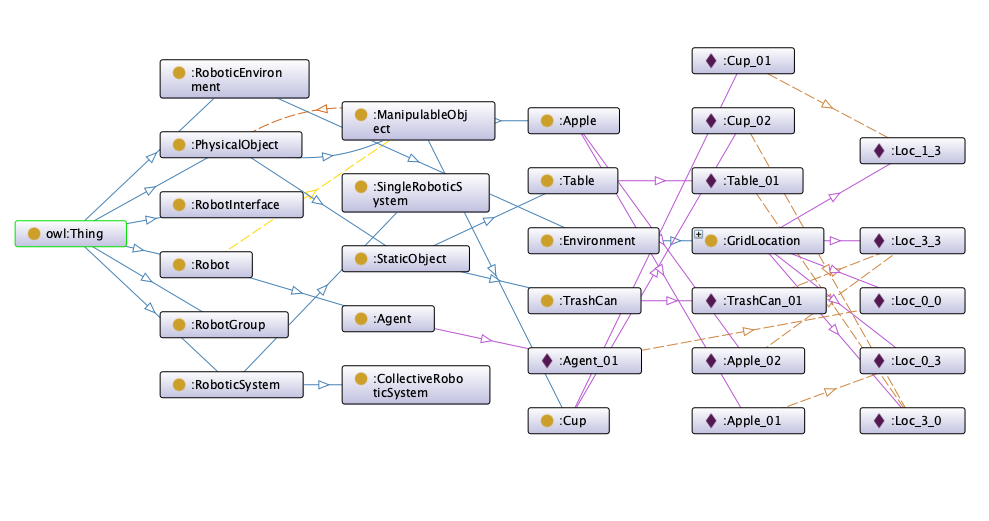
\includegraphics[width=1\textwidth]{figures/ontology_graph.png}
    \caption{Visualization of the custom Cognitive Robotics Ontology, illustrating class hierarchies and spatial relations.}
    \label{fig:ontology_graph}
\end{figure}

\begin{figure}[htbp]
    \centering
    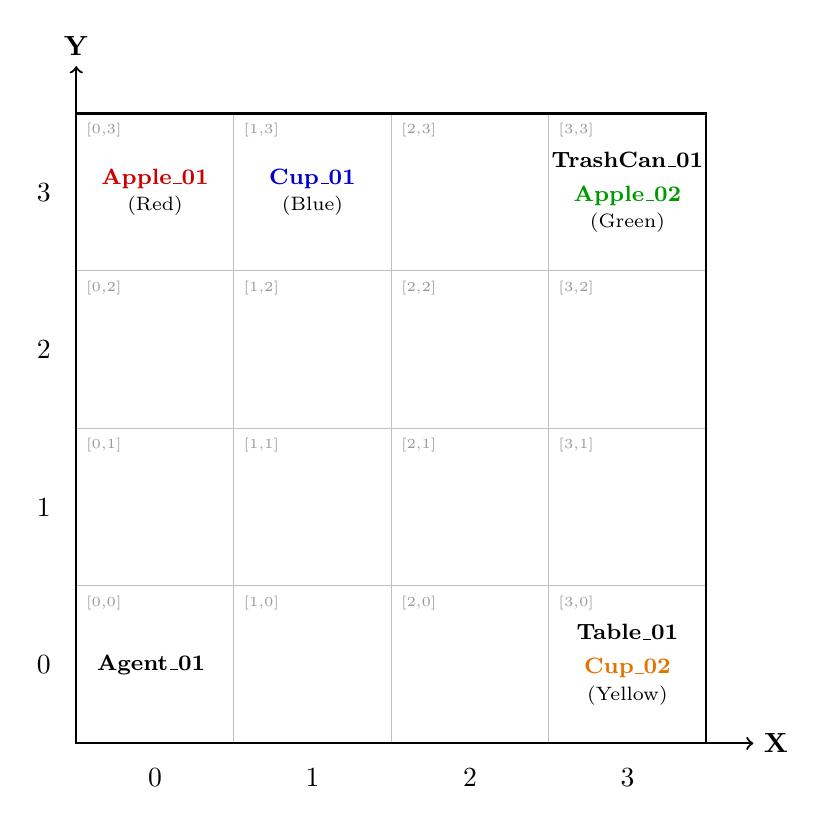
\begin{tikzpicture}[scale=2]
        
        % Grid lines
        \draw[step=1cm, gray!50, thin] (0,0) grid (4,4);
        \draw[thick] (0,0) rectangle (4,4);
        
        % X and Y axes labels
        \draw[->, thick] (0,0) -- (4.3,0) node[right] {\textbf{X}};
        \draw[->, thick] (0,0) -- (0,4.3) node[above] {\textbf{Y}};
        
        % Axis numbering
        \foreach \x in {0,1,2,3} {
            \node[anchor=north] at (\x+0.5, -0.1) {\x};
        }
        \foreach \y in {0,1,2,3} {
            \node[anchor=east] at (-0.1, \y+0.5) {\y};
        }
        
        % Coordinate labels in the top-left of every cell
        \foreach \x in {0,1,2,3} {
            \foreach \y in {0,1,2,3} {
                \node[text=gray!80, font=\tiny, anchor=north west] at (\x, \y+1) {[\x,\y]};
            }
        }
        
        % [0, 0]
        \node[align=center, font=\footnotesize] at (0.5, 0.5) {
            \textbf{Agent\_01}
        };
        
        % [0, 3]
        \node[align=center, font=\footnotesize] at (0.5, 3.5) {
            \textcolor{red!80!black}{\textbf{Apple\_01}}\\
            \scriptsize(Red)
        };
        
        % [1, 3]
        \node[align=center, font=\footnotesize] at (1.5, 3.5) {
            \textcolor{blue!80!black}{\textbf{Cup\_01}}\\
            \scriptsize(Blue)
        };
        
        % [3, 0]
        \node[align=center, font=\footnotesize] at (3.5, 0.5) {
            \textbf{Table\_01}\\[0.1cm]
            \textcolor{orange!90!black}{\textbf{Cup\_02}}\\
            \scriptsize(Yellow)
        };
        
        % [3, 3]
        \node[align=center, font=\footnotesize] at (3.5, 3.5) {
            \textbf{TrashCan\_01}\\[0.1cm]
            \textcolor{green!60!black}{\textbf{Apple\_02}}\\
            \scriptsize(Green)
        };
        
    \end{tikzpicture}
    \caption{Spatial configuration of the initial environment state extracted from the OWL/RDF ontology, mapped to a 4x4 coordinate grid.}
    \label{fig:environment_grid}
\end{figure}

\subsection{Dataset Creation}

To ensure comprehensive coverage of the domain model, Table \ref{tab:dataset_matrix} maps each instruction against the specific ontological entities, properties, and operators it explicitly triggers or evaluates. Hence, the benchmark covers the reachable success, failure, and niche control paths in the current implementations.

\newpage

\begingroup
\centering
\footnotesize
\setlength{\LTcapwidth}{\textwidth}
\renewcommand{\arraystretch}{1.7}
\begin{xltabular}{\textwidth}{@{} >{\bfseries}p{0.10\textwidth} X p{0.50\textwidth} @{}}
    \caption{Coverage-Oriented Semantic Command Dataset for Evaluation} \label{tab:dataset_matrix} \\
    \toprule
    ID & Natural Language Instruction & Gold Action Schema (from \texttt{ground\_truth.txt}) \\
    \midrule
    \endfirsthead
    
    \toprule
    ID & Natural Language Instruction & Gold Action Schema (from \texttt{ground\_truth.txt}) \\
    \midrule
    \endhead
    
    \bottomrule
    \endfoot
    
    \bottomrule
    \endlastfoot
    
    \multicolumn{3}{@{}l}{\textbf{Simple}} \\
    \midrule
    CMD-01 & Move to (2,2). & \path{move(desired-x=2; desired-y=2)} \\
    CMD-02 & Move to [-1, 5]. & \path{move(desired-x=-1; desired-y=5)} \\
    CMD-03 & Move north. & \path{move(direction=north)} \\
    CMD-04 & Move east. & \path{move(direction=east)} \\
    CMD-05 & Move south. & \path{move(direction=south)} \\
    CMD-06 & Move west. & \path{move(direction=west)} \\
    CMD-07 & Move up by 2. & \path{move(direction=north; distance=2)} \\
    CMD-08 & Move down by 3. & \path{move(direction=south; distance=3)} \\
    CMD-09 & Move forward 5 steps. & \path{move(distance=5)} \\
    \midrule
    
    \multicolumn{3}{@{}l}{\textbf{Attribute-based}} \\
    \midrule
    CMD-10 & Tell me the coordinates of the green apple. & \path{query-location(target-class=apple; target-modifiers=[green])} \\
    CMD-11 & Bring the red apple to loc\_1\_3. & \path{get(target-class=apple; target-modifiers=[red]) -> set(desired-x=1; desired-y=3)} \\
    CMD-12 & Bring the green apple to loc\_0\_0. & \path{get(target-class=apple; target-modifiers=[green]) -> set(desired-x=0; desired-y=0)} \\
    CMD-13 & Where is the yellow cup? & \path{query-location(target-class=cup; target-modifiers=[yellow])} \\
    CMD-14 & Where is the blue cup? & \path{query-location(target-class=cup; target-modifiers=[blue])} \\
    CMD-15 & Pick up the green apple. & \path{get(target-class=apple; target-modifiers=[green])} \\
    CMD-16 & Pick up the blue cup. & \path{get(target-class=cup; target-modifiers=[blue])} \\
    CMD-17 & Pick up the dirty green apple. & \path{get(target-class=apple; target-modifiers=[dirty,green])} \\
    CMD-18 & Where is cup\_02 that is blue? & \path{query-location(target-class=cup; target-modifiers=[02,blue])} \\
    CMD-19 & Where is the apple? & \path{query-location(target-class=apple)} \\
    CMD-20 & Tell me the coordinates of the red apple. & \path{query-location(target-class=apple; target-modifiers=[red])} \\
    \midrule
    
    \multicolumn{3}{@{}l}{\textbf{Spatial Relations}} \\
    \midrule
    CMD-21 & Is the yellow cup on the table? & \path{query-boolean(target-class=cup; target-modifiers=[yellow]; destination-class=table)} \\
    CMD-22 & Does the trashcan contain the green apple? & \path{query-boolean(target-class=apple; target-modifiers=[green]; destination-class=trashcan)} \\
    CMD-23 & Does the trashcan contain the red apple? & \path{query-boolean(target-class=apple; target-modifiers=[red]; destination-class=trashcan)} \\
    CMD-24 & Is the green apple on the table? & \path{query-boolean(target-class=apple; target-modifiers=[green]; destination-class=table)} \\
    CMD-25 & Is the agent next to the table? & \path{query-boolean(target-class=agent; destination-class=table)} \\
    CMD-26 & Does the table hold the green apple? & \path{query-boolean(target-class=apple; target-modifiers=[green]; destination-class=table)} \\
    CMD-27 & Are you near the trashcan? & \path{query-boolean(target-class=agent; destination-class=trashcan)} \\
    CMD-28 & Is the yellow cup inside the trashcan? & \path{query-boolean(target-class=cup; target-modifiers=[yellow]; destination-class=trashcan)} \\
    CMD-29 & Is the cup in the blue trashcan? & \path{query-boolean(target-class=cup; destination-class=trashcan; destination-modifiers=[blue])} \\
    \midrule

    \multicolumn{3}{@{}l}{\textbf{Ambiguous}} \\
    \midrule
    CMD-30 & Head towards the trashcan. & \path{move(destination-class=trashcan)} \\
    CMD-31 & Where is agent\_01 located? & \path{query-location(target-class=agent; target-modifiers=[01])} \\
    CMD-32 & What are you holding? & \path{query-inventory(target-class=agent)} \\
    CMD-33 & Drop the item. & \path{set()} \\
    CMD-34 & Pick up the table. & \path{get(target-class=table)} \\
    CMD-35 & Go over there. & \path{move()} \\
    CMD-36 & Throw it away. & \path{set(destination-class=trashcan)} \\
    CMD-37 & Grab it. & \path{get()} \\
    CMD-38 & Put it down. & \path{set()} \\
    CMD-39 & Bring it to loc\_4\_4. & \path{set(desired-x=4; desired-y=4)} \\
    CMD-40 & Put that on the table. & \path{set(destination-class=table)} \\
    CMD-41 & Put the table inside the cup. & \path{get(target-class=table) -> set(destination-class=cup)} \\
    CMD-42 & Hello robot, please be nice and pick up the green apple for me. Thanks! & \path{get(target-class=apple; target-modifiers=[green])} \\
    \midrule

    \multicolumn{3}{@{}l}{\textbf{Multi-step}} \\
    \midrule
    CMD-43 & Pick up the green apple, then tell me what you are holding. & \path{get(target-class=apple; target-modifiers=[green]) -> query-inventory(target-class=agent)} \\
    CMD-44 & Fetch the yellow cup and put it in the trashcan. & \path{get(target-class=cup; target-modifiers=[yellow]) -> set(destination-class=trashcan)} \\
    CMD-45 & Throw the red fruit into the bin. & \path{get(target-class=apple; target-modifiers=[red]) -> set(destination-class=trashcan)} \\
    CMD-46 & Put the red apple on the big table. & \path{get(target-class=apple; target-modifiers=[red]) -> set(destination-class=table; destination-modifiers=[big])} \\
    CMD-47 & Pick up the green apple, then pick up the yellow cup. & \path{get(target-class=apple; target-modifiers=[green]) -> get(target-class=cup; target-modifiers=[yellow])} \\
    CMD-48 & Pick up the green apple, then drop it. & \path{get(target-class=apple; target-modifiers=[green]) -> set()} \\
    CMD-49 & Move north, then pick up the blue cup. & \path{move(direction=north) -> get(target-class=cup; target-modifiers=[blue])} \\
    CMD-50 & Get the red apple and drop it on the table. & \path{get(target-class=apple; target-modifiers=[red]) -> set(destination-class=table)} \\
    CMD-51 & Bring the yellow cup to loc\_2\_2 and then move south. & \path{get(target-class=cup; target-modifiers=[yellow]) -> set(desired-x=2; desired-y=2) -> move(direction=south)} \\
    CMD-52 & Check if the yellow cup is on the table, then move east. & \path{query-boolean(target-class=cup; target-modifiers=[yellow]; destination-class=table) -> move(direction=east)} \\
    CMD-53 & Pick up the blue cup, drop it in the trashcan, and move west. & \path{get(target-class=cup; target-modifiers=[blue]) -> set(destination-class=trashcan) -> move(direction=west)} \\
    
\end{xltabular}
\endgroup

\subsection{Hybrid Integration}
This research explicitly decouples natural language interpretation from physical execution: neural LLMs act purely as probabilistic semantic interpreters, Ontologies provide declarative physical constraints, and Cognitive Architectures (Soar \& ACT-R) serve as the deterministic control engines executing the structured JSON logic.

\subsubsection{Shared Architecture}
All four computational pipelines are built upon a shared architectural framework that standardizes parsing, orchestration, and evaluation logic. A lightweight Python middleware decouples natural language interpretation from physical grounding, allowing the individual symbolic systems to operate solely as execution engines.

\begin{itemize}
    \item \textbf{Dataset Loader:} Systematically reads the 53 paired command/gold benchmark entries via \texttt{load\_dataset.py}.
    \item \textbf{Semantic Parser:} A 26-billion parameter LLM (\texttt{a4b} quantized for low-latency edge execution) serves as a universal semantic translator, ensuring robust zero-shot JSON schema adherence. To balance stochasticity and reproducibility, the model is queried at temperature 1.0 using deterministic seeds. Outputs are cached so all pipelines evaluate identical prompts.
    \item \textbf{Testing Harness \& KPI Computation:} A centralized driver orchestrates the execution pipelines. Per-command results, including execution traces and token usage, are encapsulated in a \texttt{PipelineResult} dataclass. The harness invokes shared functions to generate \texttt{KPIScore} evaluations, saving the outputs to \path{Pipelines/Tests/outputs/[Pipeline]/CMD-XX-RYY.json} to facilitate cross-run aggregation.
    \item \textbf{Execution Tracing \& Traceability:} To enable direct behavioral comparisons, all runtimes emit execution events normalized into a standard format. Trace markers include \texttt{[ACTION]} (physical state transitions like move, get, set), \texttt{[QUERY]} (epistemic outputs), \texttt{[SUCCESS]} (completed command sequences), \texttt{[FAILURE]} (symbolic constraint rejection), and \texttt{[STUCK]} (no-terminal-condition edge cases).
\end{itemize}

Because all execution pipelines leverage this shared state and parsing logic, the system universally inherits the following validated properties:
\begin{itemize}
    \item \textbf{Constraint-First Safety:} Rather than relying on the LLM for physical compliance, each pipeline's core symbolic technology actively detects and blocks constraint violations prior to execution. This includes rejecting out-of-bounds coordinates, manipulation of static objects, capacity limits, and empty-gripper \texttt{set} commands.
    \item \textbf{Grounded Deixis:} Ambiguous commands (e.g., "drop it" or "grab it") are resolved by reading the agent's current simulated holding state, preventing LLM hallucination or guessing.
    \item \textbf{State-Aware Querying:} Query operators strictly read the current symbolic world state to produce explicit boolean, spatial, or inventory responses.
    \item \textbf{Deterministic Termination:} Command chains are guaranteed to terminate through explicit success, failure, or stuck logic.
\end{itemize}

\subsubsection{Explainability}
Within the \textbf{LLM} semantic parser, explainability is not measured through opaque internal weights, but through explicit structural constraints. To serve as a measurable proxy for interpretability, the prompt engineering completely restricts the LLM to outputting a predefined JSON schema corresponding to actionable cognitive commands. Any misinterpretation of natural language, such as hallucinated objects or incorrect spatial routing, is immediately isolated within discrete key-value pairs (e.g., \texttt{target-class}, \texttt{desired-x}, or \texttt{destination-modifiers}) prior to physical execution. This structured mapping, combined with input-output token usage tracking, provides a clear, qualitative rubric for evaluating reliability.

In cognitive architectures like \textbf{Soar}, native debug logs evaluate the system at the micro-cognitive level, tracking every preference generation, operator application, and architectural impasse. Because the Soar architecture loops continuously until a state no-change or a predefined step-limit is triggered, the execution trace is intentionally augmented with the aforementioned standardized trace markers. This maps internal operator sequencing directly to real-world behavioral outcomes, allowing researchers to pinpoint the exact cognitive cycle where a command succeeded or was rejected.

Similarly, the \textbf{ACT-R} pipeline establishes explainability by making its modular cognitive states structurally transparent. The trace structure tracks the instantiation of declarative chunks within the goal buffer and the subsequent firing of production rules. Transparency is achieved by observing the sequential activation of these modules, enabling a clear map between symbolic mechanisms and the resulting robotic actions. By generating explicit logs of buffer transitions, the system provides a traceable proxy of how architectural constraints, such as manipulability, capacity limits, and perspective-taking, are actively enforced during execution.

\subsubsection{Error Typology}
To ensure a meaningful interpretation of system failures across the defined KPIs, any errors encountered during the text-to-action translation and symbolic execution phases are classified into a formalized taxonomy. This taxonomy distinctly separates failures of the \textbf{interpreter} from failures triggered by the \textbf{constraint system}:

\begin{itemize}
    \item \textbf{Linguistic Parsing Errors:} Failures occurring when the foundation model incorrectly maps natural language syntax to the intended JSON action schema. This includes omitted parameters, misidentified target classes, or a failure to capture explicitly stated object modifiers (e.g., ignoring "green" when instructed to fetch a "green apple").
    \item \textbf{Semantic Errors:} Instances where the generated output is syntactically valid but semantically flawed given the predefined domain mapping rules. Examples include incorrectly generating a \texttt{set} action when a \texttt{get} (pick up) action is implicitly required, or assigning physical destination parameters to an incompatible query class.
    \item \textbf{Planning Errors:} Logical sequencing failures predominantly observed in multi-step commands. While individual atomic actions may be parsed correctly, the sequence is either out of order or misses critical intermediate prerequisites (e.g., failing to generate a \texttt{get} action before attempting to \texttt{set} a requested object into a bin).
    \item \textbf{World Knowledge Errors:} Failures occurring during the symbolic execution phase rather than the linguistic parsing phase. In these cases, the command sequence is linguistically and semantically sound but violates the physical or state constraints of the simulated environment (e.g., navigating out of bounds, attempting to manipulate an unreachably distant object, or exceeding inventory capacities).
\end{itemize}

This structured classification is essential for diagnosing the specific limitations of the LLM-to-symbolic pipeline. It directly informs the granular evaluation of Interpretation Accuracy (KPI-01) by isolating text-level failures, while explaining task failures captured in the Constraint Violation Rates (KPI-05) via world-knowledge grounding.

\subsection{Pipeline A: Soar}

The Soar pipeline translates the shared JSON action schema into grounded cognitive commands. By utilizing Soar as the deterministic control system, the LLM is explicitly forbidden from producing concrete instance IDs or resolving pronouns, those tasks are delegated entirely to Soar's symbolic logic.

The Soar instantiation employs the following specialized mechanisms:
\begin{itemize}
    \item \textbf{Initialization Protocol:} The OWL/RDF world model is translated into initialization artifacts for the cognitive runtime. The environment is initialized through an explicit \texttt{init-environment} operator so that Working Memory Elements (WMEs) are operator-supported and can be safely modified by subsequent operators. Early elaboration-only patterns produced brittle behavior. Operator-supported initialization ensures robust state updates.
    \item \textbf{Knowledge Modules:} The cognitive engine is organized as modular \texttt{.soar} files implementing elaborations, proposals, applications, and safety checks. Constraint logic is enforced via elaboration-generated failure WMEs and reject rules that remove unsafe operator proposals from the decision cycle.
\end{itemize}

\subsection{Pipeline B: ACT-R}
\label{sec:actr}
This study implements a lightweight, functional Python abstraction instead of the official Lisp-based ACT-R 7 environment. This architectural adaptation was deliberately chosen to bypass the prohibitive middleware overhead of integrating legacy Lisp kernels with modern LLM APIs and JSON state trackers. Crucially, it strictly preserves ACT-R's core cognitive bottlenecks, limited-capacity buffers and declarative memory retrieval, allowing for robust evaluation of symbolic constraint handling without unnecessary sub-symbolic mathematical overhead.

The functional ACT-R pipeline enforces cognitive control through the following simulated mechanisms:
\begin{itemize}
    \item \textbf{Declarative Memory Translation:} Prior to execution, the OWL environment state is translated into an ACT-R-inspired declarative memory JSON schema. Entities and their properties are instantiated as discrete chunks (e.g., \texttt{isa apple}, \texttt{isatlocation loc\_0\_3}).
    \item \textbf{Heuristic Subsymbolic Retrieval:} Instead of calculating strict base-level learning and spreading activation equations, chunk retrieval is governed by a heuristic scoring function. This function mimics sub-symbolic activation by prioritizing semantic feature matching (e.g., checking slot values against requested modifiers like "green") and access recency/frequency. This allows the system to probabilistically resolve ambiguous, descriptive targets into explicit physical chunk IDs.
    \item \textbf{Buffer-Driven Productions:} The traditional Rete pattern-matching engine is simulated via discrete, hard-coded conditional phases operating on a fixed 50 ms cognitive cycle. The architecture utilizes four primary, single-chunk capacity buffers: \textbf{Goal} (tracking the cognitive phase), \textbf{Imaginal} (holding the parsed action schema), \textbf{Retrieval} (holding fetched declarative chunks), and \textbf{Manual} (staging executable physical commands).
\end{itemize}

Execution begins by priming the \textit{Goal} buffer with an \texttt{encode} phase and injecting the parsed JSON action sequence into the \textit{Imaginal} buffer. The system then strictly loops through sequential production phases, logging each 50 ms step. Because the system relies on limited-capacity buffers, actions cannot physically execute until necessary prerequisites are pulled from memory.

\subsection{Pipeline C: Ontologies}

The ontology pipeline executes the parsed JSON action sequence directly over the RDF state using an integrated \texttt{OntologyWorld} and \texttt{OntologyExecutor}. For each command, the runtime loads the OWL/RDF graph and builds type/superclass indices to ensure class-aware retrieval.

Entities are resolved through a deterministic scoring function over class names, descriptive modifiers, color/type slots, and current holding bias. Upon successful resolution, the system executes \path{move/get/set/query-*} actions with explicit state mutations (e.g., updating \texttt{isAtLocation} and \texttt{isHolding} relationships) and immediately emits the standardized execution trace. Execution is strictly command-sequential and halts immediately on the first failure. Because the ontology runtime directly mutates and queries RDF triples, each trace line is inherently grounded in an explicit graph operation rather than a latent model state.

\subsection{Pipeline D: LLM Baseline}

The pure LLM baseline is intentionally two-stage and fully neural at planning time. 
\begin{itemize}
    \item \textbf{Stage 1 (Parsing):} Converts natural language to constrained JSON actions using the shared parser.
    \item \textbf{Stage 2 (Planning/Execution Simulation):} A simulated executor receives an OWL-derived textual world description and the parsed JSON action sequence. It then generates an ordered trace conforming to the standardized \path{[ACTION]/[SUCCESS]/[FAILURE]} contract used by the symbolic runtimes.
\end{itemize}
The planner prompt encodes explicit \path{move/get/set/query} transition rules. Unlike the other pipelines, this baseline does not execute through an external engine or graph model. Instead, the LLM hallucinates the step-by-step execution and returns a trace list. Parses and planning token costs are computationally summed to capture the end-to-end neural reasoning overhead.

\section{Results}

\subsection{Quantitative Results}

\begin{table}[htbp]
\centering
\footnotesize
\renewcommand{\arraystretch}{1.4}
\caption{Overall Performance Across 159 Runs per Pipeline}
\label{tab:overall_results}
\begin{tabularx}{\textwidth}{@{} l *{7}{>{\centering\arraybackslash}X} @{}}
    \toprule
    \textbf{Pipeline} & \textbf{KPI-01} & \textbf{KPI-02} & \textbf{KPI-03 (s)} & \textbf{KPI-04} & \textbf{KPI-05} & \textbf{LLM Time (s)} & \textbf{Symbolic Time (s)} \\
    \midrule
    Soar     & 1.00 & 1.00 & $13.15 \pm 9.77$ & $1286 \pm 464$ & $0.283$ (45/159) & 13.04 & 0.1091 \\
    ACT-R    & 1.00 & 1.00 & $13.04 \pm 9.77$ & $1286 \pm 464$ & $0.283$ (45/159) & 13.04 & 0.0002 \\
    Ontology & 1.00 & 1.00 & $13.04 \pm 9.77$ & $1286 \pm 464$ & $0.283$ (45/159) & 13.04 & 0.0008 \\
    LLM      & 1.00 & 1.00 & $37.20 \pm 20.06$ & $5579 \pm 938$ & $0.283$ (45/159) & 37.20 & 0.0000 \\
    \bottomrule
\end{tabularx}
\end{table}

Table \ref{tab:overall_results} shows identical correctness scores but clear efficiency separation. Relative to the pure LLM baseline, Soar/ACT-R/Ontology reduce latency by approximately 64.7--65.0\% and token usage by approximately 76.9\%. This disparity in computational overhead is further detailed across the five instruction categories in Table \ref{tab:category_latency} for planning latency and Table \ref{tab:category_tokens_violations} for token consumption and constraint violation rates. Notably, multi-step commands exact the highest temporal and token costs across all architectures, though the LLM baseline's performance degrades much more severely.

\begin{table}[htbp]
\centering
\footnotesize
\renewcommand{\arraystretch}{1.4}
\caption{Category-Level Means (KPI-03, seconds)}
\label{tab:category_latency}
\begin{tabularx}{\textwidth}{@{} l *{4}{>{\centering\arraybackslash}X} @{}}
    \toprule
    \textbf{Category} & \textbf{Soar} & \textbf{ACT-R} & \textbf{Ontology} & \textbf{LLM} \\
    \midrule
    Simple          & 7.68  & 7.57  & 7.57  & 20.01 \\
    Attribute-based & 11.32 & 11.22 & 11.22 & 35.40 \\
    Spatial Relations & 11.49 & 11.38 & 11.38 & 38.41 \\
    Ambiguous       & 15.34 & 15.23 & 15.23 & 34.59 \\
    Multi-step      & 18.21 & 18.10 & 18.10 & 55.17 \\
    \bottomrule
\end{tabularx}
\end{table}

\begin{table}[htbp]
\centering
\footnotesize
\renewcommand{\arraystretch}{1.4}
\caption{Category-Level Means (KPI-04 tokens and KPI-05 violation rate)}
\label{tab:category_tokens_violations}
\begin{tabularx}{\textwidth}{@{} l *{4}{>{\centering\arraybackslash}X} @{}}
    \toprule
    \textbf{Category} & \textbf{KPI-04 Soar/ACT-R/Ontology} & \textbf{KPI-04 LLM} & \textbf{KPI-05 (all pipelines)} & \textbf{Violating Commands} \\
    \midrule
    Simple          & 1023 & 4789 & 0.556 & 5/9 \\
    Attribute-based & 1210 & 5513 & 0.000 & 0/11 \\
    Spatial Relations & 1209 & 5530 & 0.000 & 0/9 \\
    Ambiguous       & 1384 & 5456 & 0.692 & 9/13 \\
    Multi-step      & 1525 & 6477 & 0.091 & 1/11 \\
    \bottomrule
\end{tabularx}
\end{table}

\subsection{Command-Level and Qualitative Findings}

\begin{table}[htbp]
\centering
\footnotesize
\renewcommand{\arraystretch}{1.4}
\caption{All Commands with Non-Zero KPI-05 (15/53 templates)}
\label{tab:violating_commands}
\begin{tabularx}{\textwidth}{@{} 
    l 
    l 
    >{\raggedright\arraybackslash\hsize=0.85\hsize}X 
    >{\raggedright\arraybackslash\hsize=1.15\hsize}X 
    @{}}
    \toprule
    \textbf{ID} & \textbf{Category} & \textbf{Instruction} & \textbf{Dominant Error Type (Soar / ACT-R / Ontology / LLM)} \\
    \midrule
    CMD-02 & Simple & Move to [-1, 5]. & world-knowledge-error (All Pipelines) \\
    CMD-05 & Simple & Move south. & world-knowledge-error (All Pipelines) \\
    CMD-06 & Simple & Move west. & world-knowledge-error (All Pipelines) \\
    CMD-08 & Simple & Move down by 3. & world-knowledge-error (All Pipelines) \\
    CMD-09 & Simple & Move forward 5 steps. & world-knowledge-error (All Pipelines) \\
    CMD-33 & Ambiguous & Drop the item. & planning-error (All Pipelines) \\
    CMD-34 & Ambiguous & Pick up the table. & world-knowledge-error (All Pipelines) \\
    CMD-35 & Ambiguous & Go over there. & world-knowledge-error (All Pipelines) \\
    CMD-36 & Ambiguous & Throw it away. & planning-error (All Pipelines) \\
    CMD-37 & Ambiguous & Grab it. & unknown-target (Soar) / semantic-error (Others) \\
    CMD-38 & Ambiguous & Put it down. & planning-error (All Pipelines) \\
    CMD-39 & Ambiguous & Bring it to loc\_4\_4. & planning-error (All Pipelines) \\
    CMD-40 & Ambiguous & Put that on the table. & planning-error (All Pipelines) \\
    CMD-41 & Ambiguous & Put the table inside the cup. & world-knowledge-error (All Pipelines) \\
    CMD-47 & Multi-step & Pick up the green apple, then pick up the yellow cup. & world-knowledge-error (All Pipelines) \\
    \bottomrule
\end{tabularx}
\end{table}

Table~\ref{tab:violating_commands} details all 15 violating command templates using the error taxonomy defined in Section~3.3.3. The sole cross-pipeline divergence is CMD-37 (\textit{``Grab it.''}): Soar surfaces \texttt{unknown-target} while the other pipelines report \texttt{semantic-error}, an implementation-level labeling difference rather than a behavioral one. The remaining 38/53 commands produced \texttt{KPI-05 = 0} across all runs and pipelines.

\section{Discussion}

\subsection{Architectural Efficacy and Performance}
Because all four pipelines consumed a shared JSON action schema, KPI-01 and KPI-02 could not differentiate the architectures: the parser-produced sequences are identical inputs, and safe symbolic rejection of impossible commands counts as successful execution under our criteria. The core empirical differentiator is therefore \textbf{efficiency} (KPI-03 and KPI-04): offloading state reasoning to lightweight symbolic executors reduces latency by $\sim$65\% and token consumption by $\sim$77\% relative to the pure LLM planner, as detailed in Tables~\ref{tab:category_latency} and~\ref{tab:category_tokens_violations}.

\subsection{Cognitive and Theoretical Normalization}
A core analytical observation arising from this experimental setup is that the architectures yield highly uniform correctness metrics across the board. This uniform distribution is directly attributable to the system design choice where all pipelines share the same parser-generated JSON schema representation. Consequently, the empirical comparison predominantly isolates differences in computational cost and efficiency rather than behavioral variation. While the present technical execution is highly optimized, this pattern tends to structurally normalize Soar and ACT-R into functioning as relatively similar execution backends within the Python middleware. This underscores a theoretical constraint: to fully differentiate these architectures, evaluations must look beyond top-level performance boundaries and investigate how each architecture represents, schedules, and resolves symbolic queries internally.

\subsection{Limitations and Assumptions}
The following constraints affect the overarching hybrid framework rather than isolated pipelines.

The ACT-R branch relies on a custom Python implementation (\path{Pipelines/ACTR/model.py}) rather than the canonical Lisp ACT-R runtime or \texttt{pyactr}, as described in Section~3.5. While core cognitive bottlenecks are preserved, full subsymbolic activation equations and canonical conflict-resolution internals are absent.

The static 4x4 grid environment (Section~3.1) deliberately omits sensor noise, partial observability, and continuous motion kinematics. This optimally isolates text-to-action reasoning but under-represents the uncertainties and temporal dynamics inherent to physical robotic deployment.

Finally, the pure LLM baseline acts as a simulated executor. While it is strictly prompt-constrained to emit standard execution traces for comparability, any observed failures reflect the probabilistic nature of prompt-governed reasoning rather than true algorithmic state transitions. It operates under the assumption that the OWL model serves as a correct and complete world oracle, purposefully prioritizing grounded execution guarantees over broad, unconstrained linguistic expressiveness.

\section{Conclusion and Future Work}

The symbolic frameworks (Soar, ACT-R, and Ontology) consistently outperformed the pure LLM baseline on efficiency while all four pipelines achieved identical correctness scores, validating the hybrid LLM-to-symbolic pattern as the preferred architecture for grounded robotic instruction following.

Future work could expand upon these structural findings along three main axes. First, to deepen the cognitive and theoretical comparison, experimental branches could explore the distinct cognitive differences between these architectures by lifting the uniform JSON parser constraints and testing unique procedural mechanisms native to each engine.

Second, from an interface perspective, the framework would benefit from a live React or Streamlit telemetry dashboard. Such a tool could visually capture the 4x4 grid, tracking dynamic object positions, agent state trajectories, and trace execution events step-by-step for each isolated pipeline. While valuable for real-time analysis, the design and implementation of this dedicated visualization layer remained beyond the scope of this initial study.

Finally, a promising direction for bridging abstract reasoning with physical simulation involves a minimal ROS 2 integration layer. This integration would allow the validated JSON action schemas to be published directly to simulated robotic platforms, such as a TurtleBot3 operating within a Gazebo environment. Exploring this avenue would provide a valuable opportunity to evaluate the resilience of hybrid text-to-action control under realistic physics, spatial noise, and execution constraints, serving as a logical next step for validating these architectures in dynamic environments.

\newpage
\bibliographystyle{IEEEtran}
\bibliography{refs}

\end{document}